\documentclass[runningheads]{llncs}
% 'runningheads' enables the header on subsequent pages

\usepackage{booktabs} % For professional tables
\usepackage[T1]{fontenc}
\usepackage[utf8]{inputenc}
\usepackage[english]{babel}
\usepackage{orcidlink}
\usepackage{verbatim}
\usepackage{amsmath}
\usepackage{amssymb}
\usepackage{graphicx}
\usepackage{algorithm}
\usepackage{algpseudocode}
\usepackage{hyperref}
\usepackage[margin=1in]{geometry}
\usepackage{tikz}
\usetikzlibrary{shapes, arrows.meta, positioning, calc, fit, shadows}

% Hyperlink setup
\hypersetup{
    colorlinks=true,
    linkcolor=blue,
    filecolor=magenta,      
    urlcolor=cyan,
    citecolor=blue,
}

% Professional Color Palette
\definecolor{primary}{RGB}{70, 130, 180}    % Steel Blue
\definecolor{secondary}{RGB}{255, 165, 0}   % Orange
\definecolor{accent}{RGB}{46, 139, 87}      % Sea Green
\definecolor{neutral}{RGB}{240, 240, 240}   % Light Gray

\begin{document}

\title{Heuristic-Based Agent to Solve The Online Three-Dimensional Container Loading Problem}

\author{Juan Sebasti\'an Herrera-Cobo\inst{1} \orcidlink{0000-0001-6781-6379} \and
David Álvarez-Martínez\inst{2}}

\institute{Independent Researcher, Berlin 10317, Germany
\email{sebashc\_3712@hotmail.com} \and
Los Andes University, Bogotá D.C. 111711, Colombia
\email{d.alvarezm@uniandes.edu.co}}

\maketitle

\begin{center}
Submitted to special session Learning to Optimize: RL as an optimizer
\end{center}

\begin{abstract}
The rapid growth of the global economy, driven significantly by e-commerce and complex logistics systems, creates an urgent need for increased process automation. Building upon previous heuristic-based approaches, this study proposes a Deep Reinforcement Learning (DRL) framework to address the Online Three-Dimensional Container Loading Problem (OCLP). We introduce a Dueling Deep Q-Network (DQN) agent that integrates a novel auxiliary Feasibility Masking mechanism to optimize space utilization. Unlike traditional methods relying solely on fixed logic, the proposed agent utilizes height maps, box dimensions, and buffer contents to represent the state. The agent dynamically selects the optimal placement heuristic (e.g., stacking, best-fit, corner-based) or explicitly defers the current item to a limited-capacity buffer for each time step, while an auxiliary mask head predicts and prunes invalid actions to accelerate training convergence and ensure physical stability. Computational experiments demonstrate that this hybrid approach, combining the adaptability of deep learning with established heuristics, improves volumetric efficiency and generalization in automated environments.

\keywords{Deep Reinforcement Learning \and Dueling DQN \and Feasibility Masking \and Online 3D Container Loading \and Heuristics.}
\end{abstract}

\section{Introduction}

Three-dimensional loading decisions are at the core of modern fulfillment and warehousing operations, where items must be placed in a container under strict geometric and operational constraints. In many automated settings, items arrive sequentially on a conveyor or at a robotic cell, and the system must decide in real-time whether and where to place each item. Unlike offline bin packing, where all items are known \textit{a priori}, the online variant requires immediate placement decisions without knowledge of future arrivals. This constraint significantly increases complexity, as purely greedy strategies often lead to suboptimal long-term space utilization.

We consider a single rectangular container of fixed dimensions. At each arrival, the system observes the current container surface—represented as height map and the dimensions of the incoming item. The decision is to place the item while enforcing non-overlap, boundary, and stability constraints. We study the fixed orientation variant and evaluate the impact of incorporating a limited-capacity buffer mechanism.

Since automated packing cells are increasingly deployed under a Robots-as-a-Service (RaaS) model, the resulting policies must be industry-agnostic, remaining effective across highly heterogeneous item distributions without per-deployment calibration. Consequently, the policy must generalize to instances whose size distributions may differ substantially from those seen during training.

We propose a hybrid decision framework that maintains geometric placement logic via a portfolio of classical heuristics while learning \emph{which heuristic to apply} at each step. Concretely, we train a Dueling Deep Q-Network (DQN) agent \cite{Mnih2015NatureDQN,Wang2016Dueling} that maps the container state, current item features, and buffer contents to a discrete action, selecting one among several placement heuristics or deferring the item to a buffer. To prevent wasted learning signals on infeasible decisions, we integrate a feasibility masking mechanism that prunes actions incapable of producing valid placements.

This paper makes the following contributions:
\begin{itemize}
    \item We introduce a hybrid DRL policy that learns to select among a compact portfolio of placement heuristics and an explicit buffer-deferral action, avoiding the complexity of a large continuous placement action space while integrating active buffer management into the decision process.
    \item We integrate feasibility masking to eliminate invalid heuristic actions at decision time, improving learning efficiency in constrained packing environments.
    \item We evaluate the resulting agent on synthetic and literature-derived instance families, comparing it against representative heuristic and learning-based baselines.
\end{itemize}

The remainder of the paper is organized as follows: Section~2 reviews related literature. Section~3 formalizes the problem and constraints. Sections~4--5 describe the reinforcement learning formulation and network architecture. Section~6 presents the experimental evaluation, and Section~7 concludes.

\section{Literature Review}
\label{sec:literature}
This section surveys literature relevant to our setting: online single-container 3D loading under practical constraints, focusing on learning-based decision policies and optional buffering.

Cutting-and-packing problems cover a wide range of objectives and operational assumptions. A central distinction is whether the goal is to minimize the number of containers (bin packing) or to maximize packed volume in a single container (knapsack/single-container loading) \cite{Wascher2007}. Realistic container loading also incorporates operational constraints such as orientation rules, stability requirements, and handling constraints \cite{BortfeldtWascher2013Constraints}. These practical constraints motivate solution approaches that explicitly account for feasibility during decision-making.

Online packing differs from offline loading because decisions must be made sequentially. This is particularly impactful in three dimensions, where early placements may create unusable cavities or induce fragmentation. Zhao et al.~\cite{zhao} address this setting with a constrained Deep Reinforcement Learning (DRL) approach that predicts feasibility and selects placements from a discretized set of candidate actions. Huertas et al.~\cite{david} extend the problem by incorporating buffering and repacking variants, though their solution remains heuristic-driven rather than learned.

Learning-based approaches must reconcile adaptivity to diverse sequences with strict feasibility under geometric and stability constraints. While Zhao et al.~\cite{zhao} combine constrained RL with feasibility prediction, their policy operates over a discretized geometric space that can remain prohibitively large.

Our work follows a different design: instead of learning geometric placements directly, we learn a high-level heuristic selection policy. This reduces the action space to a small discrete set while leveraging established placement heuristics. We apply feasibility masking so the agent only compares actions that can generate valid placements.

Table~\ref{tab:literature} summarizes representative related works.

\begin{table}[t]\small
\centering
\caption{Representative literature on online single-container 3D loading.}
\label{tab:literature}
\setlength{\tabcolsep}{3pt}
\renewcommand{\arraystretch}{1.05}
\begin{tabular}{p{0.5cm}p{2.8cm}p{2.2cm}p{1.5cm}p{4.2cm}}
\toprule
Ref. & Setting & Decisions & Method & Limitation vs. our work \\
\midrule
\cite{Ali2024} & Semi-online 3D heuristics & Heuristic choice & Heuristics & No DRL masking \\
\cite{Ha2017} & Online 3D dynamic arrivals & Place by rule & Heuristic & Fixed logic; no learning \\
\cite{david} & Online single-container & Place/defer & Heuristics & No learned policy \\
\cite{zhao} & Online 3D packing & Discretized placements & Constrained DRL & Geometric action space \\
\cite{Zhang2024} & Online 3D with waiting & Place/defer & DRL & No heuristic-portfolio \\
\cite{Xiong2023} & Robot packing & Reliable placements & DRL & No heuristic selection \\
\cite{Song2023} & Online 3D pack/unpack & Pack and repack & DRL & Different action model \\
\cite{Wong2024} & Online 3D optimization & RL + heuristics & Deep Q-learning & No feasibility masking \\
\bottomrule
\end{tabular}
\end{table}

\section{Problem Definition}

This section describes the Online Three-Dimensional Container Loading Problem (OCLP), including the physical setup, decision process, and constraints.

\subsection{Packing Scene}
The packing environment consists of a single rectangular container with fixed internal dimensions $L \times W \times H$. Items arrive sequentially from an external source and must be placed inside this container. The container uses a right-handed coordinate system with the origin at one corner: the $x$-axis runs along $L$, the $y$-axis along $W$, and the $z$-axis along $H$. The floor lies at $z = 0$.

Each item $i$ is a rectangular cuboid with dimensions $(l_i, w_i, h_i)$. Items may be rotated about the vertical axis (swapping $l_i$ and $w_i$), but vertical flipping is prohibited—a \emph{this side up} constraint reflecting practical requirements such as fragility or weight distribution. The effective base dimensions become $(l'_i, w'_i)$, while $h_i$ remains fixed. A placed item $i$ at position $(x_i, y_i, z_i)$ occupies the region $[x_i, x_i + l'_i] \times [y_i, y_i + w'_i] \times [z_i, z_i + h_i]$.

\subsection{Online Arrival and Decision Process}
Items arrive one at a time in an unknown order. At each time step $t$, the system observes the current item dimensions $(l_t, w_t, h_t)$ and the collection of available empty spaces, then makes an irrevocable decision: place the item or defer it to the buffer.

\subsection{Buffer Mechanism}
The system may employ a limited-capacity buffer of size $K$. When $K > 0$, deferring an item to the buffer is modeled as an explicit agent action rather than a passive fallback. At each time step, the agent may choose to defer the current item to the buffer instead of placing it immediately, allowing the item to be revisited later once future placements have created more favorable configurations. The buffer operates as a random-access store. After the item stream is exhausted, the agent attempts to place all buffered items in order using the placement heuristics. If the buffer is full and the current item can neither be placed nor deferred, the episode terminates. Without buffering ($K = 0$), the episode terminates immediately when an item admits no feasible placement.

\subsection{Geometric Constraints}
Every placement must satisfy two geometric requirements:
\begin{enumerate}
    \item \textbf{Boundary constraints:} Ensure the item fits entirely within the container: $0 \leq x_i$, $x_i + l'_i \leq L$, and analogously for the $y$ and $z$ axes with bounds $W$ and $H$.
    \item \textbf{Non-overlap constraints:} Require that any two placed items $i$ and $j$ occupy disjoint regions. This holds if and only if they are separated along at least one axis—that is, $x_i + l'_i \leq x_j$ or $x_j + l'_j \leq x_i$ (separation in $x$), and similarly for $y$ and $z$.
\end{enumerate}

\subsection{Stability Constraint}
Placements must satisfy a physical stability requirement. We enforce a \emph{minimum support coverage} rule: the base of each item must be supported over a sufficient fraction of its area. Let $A_{\text{base}}(i) = l'_i \cdot w'_i$ and let $A_{\text{sup}}(i)$ be the portion resting on the floor or top faces of other items. A placement is stable if:
\begin{equation}
    A_{\text{sup}}(i) \geq \alpha \cdot A_{\text{base}}(i),
\end{equation}
where $\alpha = 0.6$ (60\% minimum support).

\subsection{Objective}
The goal is to maximize volumetric utilization:
\begin{equation}
    U = \frac{\sum_{i \in \mathcal{P}} l_i \cdot w_i \cdot h_i}{L \cdot W \cdot H},
\end{equation}
where $\mathcal{P}$ denotes successfully placed items.

\section{Reinforcement Learning Structure}
We formulate the problem as a Markov Decision Process (MDP) defined by the tuple $(S, A, R, P, \gamma)$.

\subsection{State Space ($S$)}
The state $s_t$ is a composite representation capturing the container's geometry, the current item, and heuristic feasibility information. It consists of two components:

\begin{enumerate}
    \item \textbf{Height Map ($\mathbf{H}_t$)}: A grid $\mathbf{H}_t \in \mathbb{R}^{L \times W}$ representing the current stacking height at every coordinate $(x, y)$. This provides a dense spatial representation of the container's surface profile.
    \item \textbf{Vector Features ($\mathbf{v}_t$)}: A feature vector $\mathbf{v}_t \in \mathbb{R}^{3 + 3K + 6}$ containing:
    \begin{itemize}
        \item Normalized item dimensions: $(l_t/L, w_t/W, h_t/H_{max})$.
        \item \textbf{Buffer Contents}: The normalized dimensions of each item currently in the buffer, represented as $K$ triplets $(l_j/L, w_j/W, h_j/H_{max})$ for $j = 1, \dots, K$. Empty buffer slots are zero-padded. This encoding allows the agent to condition its deferral decisions on the current buffer composition.
        \item \textbf{Heuristic Proxy Scores}: A set of six scalars $\{s_{1}, \dots, s_{6}\}$ derived from the auxiliary mask prediction (see Section~\ref{sec:mask_bias}). The first five scores indicate the predicted feasibility confidence for the placement location chosen by each heuristic. The sixth score estimates the value of deferring the current item, computed as a function of the best heuristic confidence and buffer occupancy.
    \end{itemize}
\end{enumerate}

\subsection{Action Space ($A$)}
Rather than learning exact placement coordinates, the agent selects from a discrete set of $|A| = 5 + \mathbb{I}(K > 0)$ high-level actions: five placement heuristics and, when a buffer is available ($K > 0$), a sixth action for explicit buffer deferral. Each heuristic encapsulates a distinct packing strategy: given the current item (with effective dimensions $l'$, $w'$, $h$) and the list of feasible empty spaces $ES$, the heuristic deterministically computes a placement position $(x, y, z)$ according to its scoring criterion. This design reduces the action space from a high-dimensional continuous domain to a small discrete set while leveraging well-established packing logic.  With this smaller, discretized action space, the agent is incentivized to focus on finding robust, high-level policies—learning \textit{how} to pack and \textit{when} to defer—rather than searching for ``magical spots'' in the coordinate space. By abstracting the exact placement to heuristics and modeling deferral as an explicit decision, we prevent the agent from overfitting to specific coordinate patterns that do not generalize, allowing it to navigate the optimization landscape more effectively.

Let $\mathcal{F} \subseteq ES$ denote the subset of empty spaces where the current item can be feasibly placed (satisfying boundary, non-overlap, and stability constraints). Each heuristic $a \in A$ defines a scoring function $\sigma_a(e)$ over candidate spaces $e \in \mathcal{F}$, and selects the placement that optimizes this score. The five heuristics are:

\paragraph{1. Stacking Heuristic.}
This heuristic prioritizes vertical consolidation by placing items as high as possible within the container. It selects the empty space with the maximum base height:
\begin{equation}
    e^* = \arg\max_{e \in \mathcal{F}} \; z_e.
\end{equation}
By building upward from existing items, stacking creates flat, consolidated layers that preserve contiguous floor-level space for larger items arriving later. This strategy is particularly effective when items have similar base dimensions.

\paragraph{2. Best-Fit Heuristic.}
Best-fit minimizes the vertical residual space above the placed item, seeking locations where the item nearly reaches the container ceiling or the base of an item above. The scoring function is:
\begin{equation}
    e^* = \arg\min_{e \in \mathcal{F}} \; (H_e - h),
\end{equation}
where $H_e$ is the available height of empty space $e$ and $h$ is the item height. This heuristic reduces vertical fragmentation by filling tall gaps with appropriately sized items, leaving minimal unusable overhead space.

\paragraph{3. Semi-Perfect-Fit Heuristic.}
This heuristic targets placements that minimize local volumetric waste by considering fit quality across all three dimensions. It scores each candidate space by the sum of dimensional residuals:
\begin{equation}
    e^* = \arg\min_{e \in \mathcal{F}} \; \bigl[(L_e - l') + (W_e - w') + (H_e - h)\bigr].
\end{equation}
A placement is considered ``semi-perfect'' when the item dimensions closely match the empty space dimensions, leaving little residual volume. This approach reduces fragmentation by consuming spaces that would otherwise be difficult to fill with future items.

\paragraph{4. Corner-Based Heuristic.}
The corner-based heuristic maximizes contact between the placed item and existing boundaries---container walls or faces of previously placed items. Let $c(e)$ denote the number of item faces that would be flush against a wall or neighbor when placed in space $e$. The selection criterion is:
\begin{equation}
    e^* = \arg\max_{e \in \mathcal{F}} \; c(e).
\end{equation}
Placements in corners (contact on three faces) are preferred over edge placements (two faces), which in turn are preferred over interior placements. This strategy consolidates items against boundaries, preserving large contiguous regions in the container interior for future arrivals.

When the agent selects a heuristic action $a \in \{1, \dots, 5\}$, the corresponding heuristic is executed on the current state. If the heuristic finds a valid placement, the item is placed and the environment transitions to the next state. Actions corresponding to heuristics that cannot produce any feasible placement are masked prior to selection (see Section~\ref{sec:mask}), ensuring the agent only chooses among currently viable strategies. The buffer defer action ($a = 6$), when available, is masked when the buffer is full ($|\text{buffer}| \geq K$).

\paragraph{5. Complex Fit Heuristic.}
This heuristic prioritizes the "replicability" of a placement by analyzing the geometry of the remaining empty space. It seeks positions where the distance to the nearest obstacle (boundary or taller item) is an exact multiple of the item's dimensions, thereby minimizing non-usable "residue" gaps. The optimal placement $e^*$ is selected by maximizing the modular fit in both lateral dimensions:
\begin{equation}
e^* = \arg\max_{e=(x,y) \in \mathcal{F}} \left( \mathbb{I}\big(L_x \pmod w = 0\big) + \mathbb{I}\big(L_y \pmod d = 0\big) \right) + \epsilon(e),
\end{equation}
where $L_x$ and $L_y$ represent the total available length from the placement coordinate to the nearest boundary along the $x$ and $y$ axes, $w$ and $d$ are the item's dimensions, $\mathbb{I}$ is the indicator function, and $\epsilon(e)$ serves as a tie-breaker based on contact maximization and vertical minimization. By enforcing modularity, this strategy facilitates dense packing patterns for batches of identical items.

\paragraph{6. Buffer Defer Action ($K > 0$ only).}
When a buffer of capacity $K$ is available, the agent may select a sixth action that defers the current item to the buffer instead of placing it immediately. This action is masked (set to $-\infty$ in the Q-values) when the buffer is full, ensuring the agent only considers deferral when capacity remains. The buffer defer action is not available during the buffer-emptying phase that occurs after the item stream is exhausted. By modeling deferral as an explicit learned decision rather than a passive fallback, the agent can strategically postpone items that are difficult to place in the current configuration, reserving them for later when the container surface may offer more favorable placement opportunities.

\subsection{Space-Aware Heuristic Scoring}
\label{sec:space_aware}

A distinguishing feature of our approach is that each placement heuristic incorporates a \emph{space preservation} criterion. The heuristics evaluate candidate placements based on the quality of the maximal empty spaces that would remain after placement. We define the \emph{average maximal space volume} after placing item $i$ at position $(x, y, z)$ as:
\begin{equation}
    \bar{V}_{ES}(x, y, z) = \frac{1}{|ES'|} \sum_{e \in ES'} L_e \cdot W_e \cdot H_e,
\end{equation}
where $ES'$ denotes the updated list of maximal empty spaces after the placement. Placements that yield higher $\bar{V}_{ES}$ preserve larger, more usable regions for subsequent items.

Each heuristic $a$ evaluates candidate empty spaces using a composite score that balances the primary criterion $\sigma_a(e)$ with the space preservation objective. For a candidate placement in empty space $e$, the effective score becomes:
\begin{equation}
    \tilde{\sigma}_a(e) = \sigma_a(e) + \omega \cdot \bar{V}_{ES}(e),
\end{equation}
where $\omega > 0$ weights the importance of preserving large empty spaces. This formulation encourages placements that:

\begin{itemize}

    \item Avoid creating small, fragmented cavities that are difficult to fill

    \item Maintain contiguous regions suitable for larger future items

    \item Reduce geometric waste from irregular residual spaces

\end{itemize}


Myopic placement strategies that only consider immediate fit quality often fragment the container, leaving no room for larger items arriving later. By leveraging the maximal space definition within both the reward structure and the feasibility mask, we obviate the need for computationally expensive look-ahead simulations, such as those found in Monte Carlo Tree Search approaches \cite{zhao}. Our aim is to maintain the model's logic as efficient and lightweight as possible, deriving implicit foresight from the geometric representation rather than explicit simulation. This allows the agent to balance immediate volume gain against long-term space preservation. The principle is especially important for heterogeneous sequences: preserving a few large empty spaces accommodates a wider range of future item sizes than many small fragmented spaces of equivalent total volume.

\subsection{Reward Function ($R$)}
The reward function balances volumetric efficiency with surface flatness to encourage stable stacks and efficient buffer usage. For a successful heuristic placement at time $t$:
\begin{equation}
    r_t = \frac{V_{item}}{V_{container}} + 0.1 \cdot \left( \frac{F_{new} - F_{old}}{L \cdot W} \right) + 0.02 \cdot \frac{K - |\text{buffer}|}{K},
\end{equation}
where $F$ is the "Maximal Flat Area" metric calculated on the height map, and the third term is a buffer occupancy bonus that rewards keeping buffer capacity available (applied only when $K > 0$). This bonus incentivizes the agent to place items directly when possible rather than relying excessively on deferral.

When the agent selects the buffer defer action, the reward penalizes deferral proportionally to buffer occupancy:
\begin{equation}
    r_t^{\text{defer}} = -0.05 - 0.1 \cdot \frac{|\text{buffer}|}{K},
\end{equation}
producing a penalty ranging from $-0.05$ (empty buffer) to $-0.15$ (nearly full buffer).

If the agent attempts a heuristic action that yields no valid placement, or defers when the buffer is full, a terminal penalty is applied:
\begin{equation}
    r_t = -0.5 \quad (\text{if invalid or buffer overflow}).
\end{equation}

\section{Neural Network Architecture}

This section provides a detailed description of the neural network architecture, input processing, and hyperparameters to enable full reproducibility. The agent employs a Dueling Deep Q-Network (DQN) with multi-modal input processing and an auxiliary mask prediction head.

\subsection{Input Representation and Preprocessing}
The network receives three distinct input modalities corresponding to the current container state and the item to be packed.

\paragraph{1. Height Map ($\mathbf{H}$)}
The agent utilizes a grid-based height map representation of the pallet. For a pallet of size $L \times W$, the state is represented as a matrix $\mathbf{H} \in \mathbb{R}^{L \times W}$, where each entry $h_{ij}$ represents the current stack height at position $(i, j)$. The height map is normalized by the maximum container height $H_{max}$:
\begin{equation}
    \tilde{\mathbf{H}} = \frac{\mathbf{H}}{H_{max}}.
\end{equation}
This normalized map is treated as a single-channel image $(1, L, W)$ and processed via the convolutional encoder.

\paragraph{2. Item Dimensions ($\mathbf{d}$)}
The dimensions of the current box to be packed are given as a vector $\mathbf{d} = (l, w, h)$. These are normalized relative to the container dimensions:
\begin{equation}
    \tilde{\mathbf{d}} = \left( \frac{l}{L}, \frac{w}{W}, \frac{h}{H_{max}} \right).
\end{equation}

\paragraph{3. Buffer Contents ($\mathbf{b}$)}
When a buffer of capacity $K$ is available, the normalized dimensions of each buffered item are concatenated into a fixed-size vector $\mathbf{b} \in \mathbb{R}^{3K}$. For each buffered item $j$, the triplet $(l_j/L, w_j/W, h_j/H_{max})$ is included in order; empty buffer slots are zero-padded. This representation provides the agent with explicit knowledge of which items have been deferred, enabling informed decisions about whether to defer the current item or place it immediately.

\subsection{Network Architecture}
The agent utilizes a custom \textit{ProNet} architecture designed to process the hybrid state representation. The network consists of two input branches that fuse into a shared representation for the value and advantage heads, while a separate mask head branches directly from the spatial features.

\subsubsection{Spatial Branch (Height Map)}
The normalized height map $\tilde{\mathbf{H}}$ ($1 \times L \times W$) is processed by a 3-layer Convolutional Neural Network (CNN). Unlike standard increasing-channel architectures, we utilize a uniform feature depth to preserve spatial resolution for the mask head:
\begin{enumerate}
    \item \textbf{Conv2D}: $1 \to 64$ channels, $3\times3$ kernel, padding 1, ReLU.
    \item \textbf{Conv2D}: $64 \to 64$ channels, $3\times3$ kernel, padding 1, ReLU.
    \item \textbf{Conv2D}: $64 \to 64$ channels, $3\times3$ kernel, padding 1, ReLU.
    \item \textbf{Flatten}: Output vector size $64 \cdot L \cdot W$.
\end{enumerate}

\subsubsection{Vector Branch}
The vector input $\mathbf{v}_t \in \mathbb{R}^{3 + 3K + 6}$ (Item Dims, Buffer Contents, Proxy Scores) is processed by a Multi-Layer Perceptron (MLP):
\begin{itemize}
    \item Linear ($(3 + 3K + 6) \to 128$) $\to$ ReLU $\to$ Linear ($128 \to 128$) $\to$ ReLU.
\end{itemize}
The wider hidden layers (128 units) accommodate the additional buffer information and provide sufficient capacity for learning buffer-aware policies.

\subsubsection{Heads and Fusion}
The flattened spatial features and the processed vector features are concatenated to form the latent vector $\mathbf{z}$.
\begin{itemize}
    \item \textbf{Value Head $V(s)$}: Linear($\text{size}(\mathbf{z}) \to 512$) $\to$ ReLU $\to$ Linear($512 \to 1$).
    \item \textbf{Advantage Head $A(s,a)$}: Linear($\text{size}(\mathbf{z}) \to 512$) $\to$ ReLU $\to$ Linear($512 \to |A|$).
\end{itemize}

\subsubsection{Auxiliary Mask Head}
\label{sec:mask} 
To accelerate training, an auxiliary mask head predicts a pixel-wise placement quality map. This head branches \textit{only} from the spatial feature map $\Phi_s \in \mathbb{R}^{64 \times L \times W}$ (extracted by the three-layer CNN encoder), ensuring the prediction relies solely on the current height map geometry. The network structure is:
\begin{itemize}
    \item Flatten($64 \cdot L \cdot W$) $\to$ Linear($64 \cdot L \cdot W \to 512$) $\to$ ReLU
    \item Linear($512 \to 2 \cdot L \cdot W$) $\to$ Reshape($2, L, W$)
\end{itemize}
The output provides logits for two rotation channels ($0^\circ, 90^\circ$) across the $L \times W$ grid. During training, this head is supervised using a Binary Cross Entropy (BCE) loss with a weight of $\lambda=0.15$. The ground-truth mask is generated dynamically by identifying placement positions that satisfy a 60\% surface support constraint and maximize the average flat area of the resulting stack.

\paragraph{Design Iteration:} The representation of the mask target underwent several design iterations, specifically comparing binary versus continuous (float) targets. While a floating-point representation theoretically allows the model to learn subtle physical gradients, empirical testing revealed that it significantly slowed convergence. The model spent excessive capacity approximating the physics engine rather than optimizing high-level policy decisions. Consequently, a binary mask was adopted to provide a sharper, more efficient learning signal.

\subsection{Loss Function}
The total loss is a weighted sum of the Deep Q-Learning loss and the auxiliary mask loss:
\begin{equation}
    \mathcal{L}_{total} = \text{SmoothL1}(Q, Y_{target}) + \beta \cdot \text{BCEWithLogits}(\hat{M}, M_{GT}),
\end{equation}
where $\beta=0.15$. The mask loss is calculated only for steps where a valid box exists ($\sum \text{dims} > 0$) and the selected action is a placement heuristic (not the buffer defer action), since deferral has no spatial placement target.

\begin{figure}[ht]
    \centering
    \resizebox{\textwidth}{!}{
    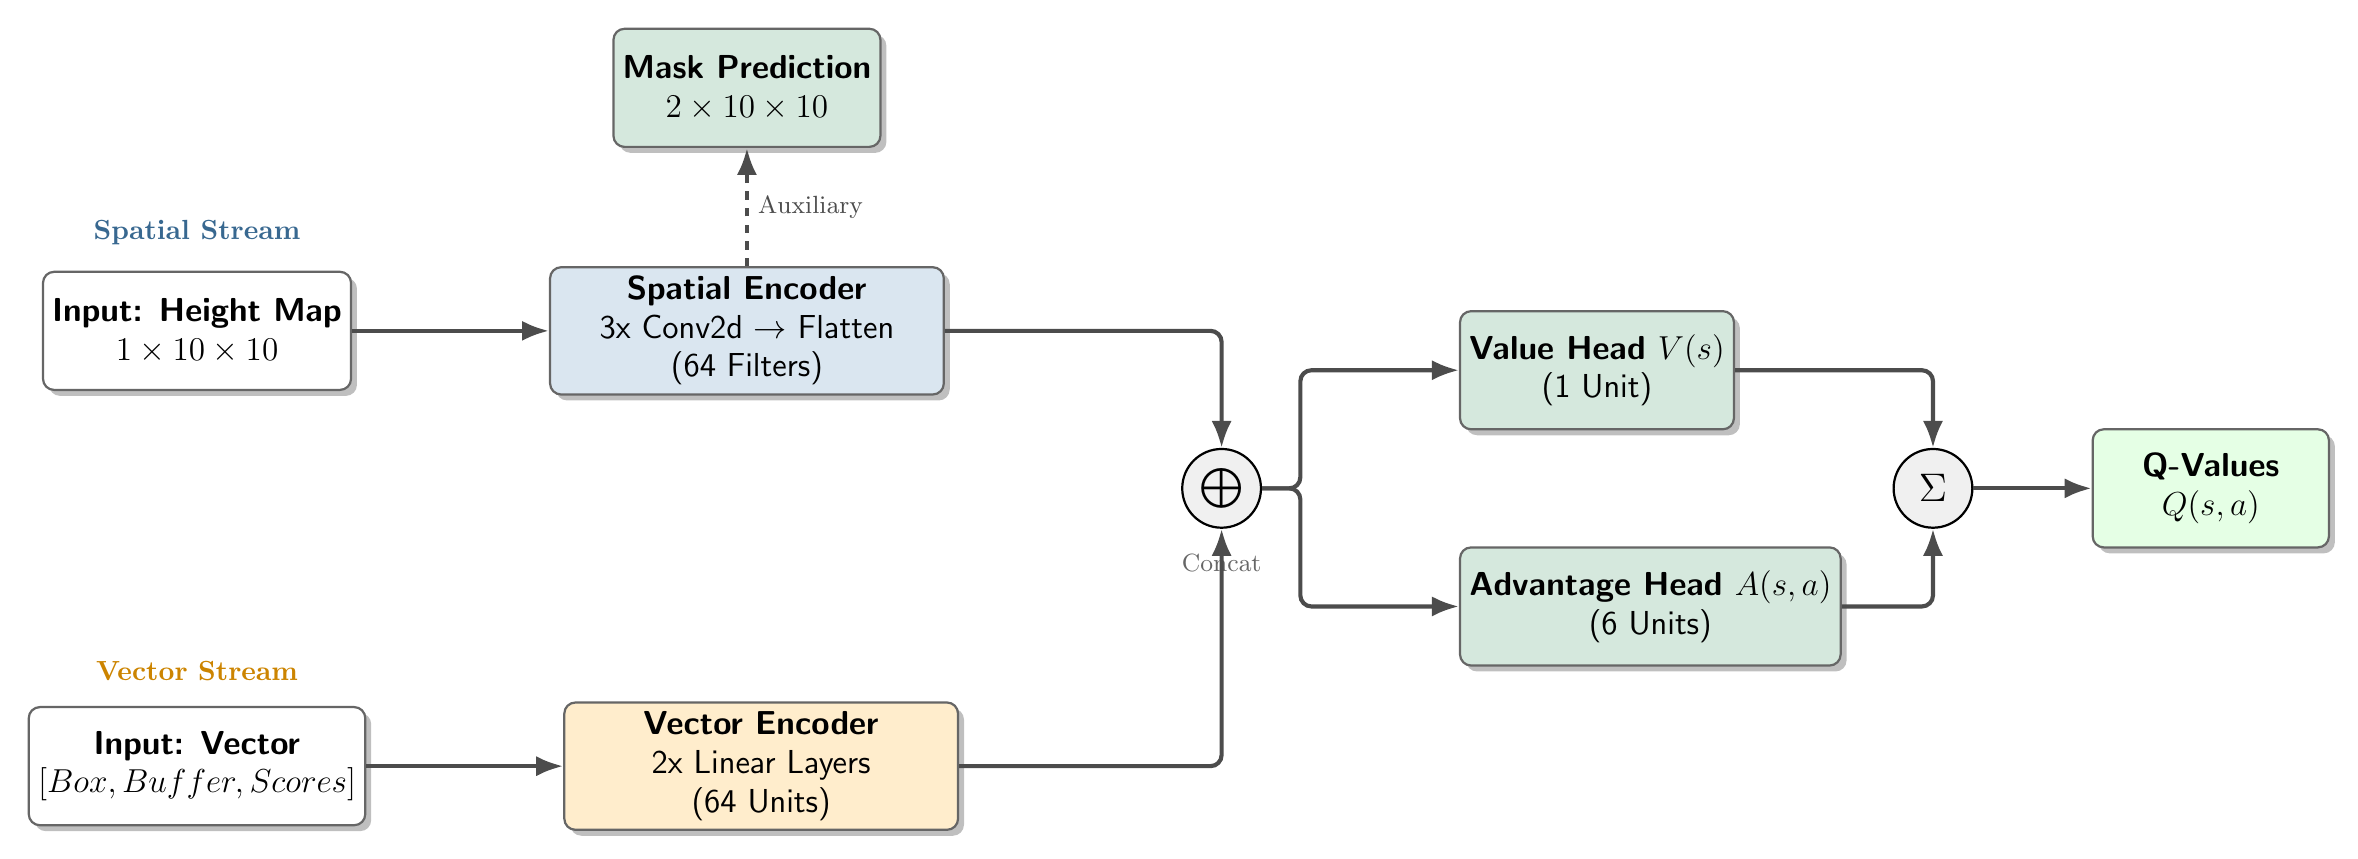
\begin{tikzpicture}[
        node distance=2cm and 2cm,
        font=\sffamily\large, % Larger font
        % Styles
        block/.style={
            rectangle, 
            draw=black!60, 
            thick, 
            rounded corners, 
            minimum height=1.5cm, 
            minimum width=3cm, 
            align=center, 
            fill=white, 
            drop shadow
        },
        encoder/.style={block, fill=primary!20},
        mlp/.style={block, fill=secondary!20},
        head/.style={block, fill=accent!20},
        op/.style={circle, draw, thick, fill=neutral, minimum size=1cm, inner sep=0pt},
        conn/.style={-Latex, line width=1.5pt, draw=black!70, rounded corners}
    ]

    % ==============================
    % 1. INPUTS
    % ==============================
    \node[block] (input_spatial) {
        \textbf{Input: Height Map}\\
        $1 \times 10 \times 10$
    };

    \node[block, below=4cm of input_spatial] (input_vector) {
        \textbf{Input: Vector}\\
        $[Box, Buffer, Scores]$
    };

    % ==============================
    % 2. ENCODERS
    % ==============================
    \node[encoder, right=2.5cm of input_spatial, minimum width=5cm] (spatial_enc) {
        \textbf{Spatial Encoder}\\
        3x Conv2d $\to$ Flatten\\
        (64 Filters)
    };

    \node[mlp, right=2.5cm of input_vector, minimum width=5cm] (vec_enc) {
        \textbf{Vector Encoder}\\
        2x Linear Layers\\
        (64 Units)
    };

    % ==============================
    % 3. MASK HEAD (Auxiliary)
    % ==============================
    \node[head, above=1.5cm of spatial_enc] (mask_head) {
        \textbf{Mask Prediction}\\
        $2 \times 10 \times 10$
    };
    
    \draw[conn, dashed] (spatial_enc.north) -- (mask_head.south) node[midway, right, font=\small, text=black!70] {Auxiliary};

    % ==============================
    % 4. FUSION
    % ==============================
    \node[op, right=3cm of spatial_enc, yshift=-2cm] (concat) {\Large $\bigoplus$};
    \node[below=0.2cm of concat, font=\small, text=black!60] {Concat};

    \draw[conn] (spatial_enc.east) -| (concat.north);
    \draw[conn] (vec_enc.east) -| (concat.south);

    % ==============================
    % 5. DUELING HEADS
    % ==============================
    \node[head, right=2.5cm of concat, yshift=1.5cm] (val_head) {
        \textbf{Value Head $V(s)$}\\
        (1 Unit)
    };

    \node[head, right=2.5cm of concat, yshift=-1.5cm] (adv_head) {
        \textbf{Advantage Head $A(s,a)$}\\
        (6 Units)
    };

    \draw[conn] (concat) -- ++(1,0) |- (val_head);
    \draw[conn] (concat) -- ++(1,0) |- (adv_head);

    % ==============================
    % 6. OUTPUT
    % ==============================
    \node[op, right=2cm of val_head, yshift=-1.5cm] (sum) {\Large $\Sigma$};
    \node[block, right=1.5cm of sum, fill=green!10] (final_q) {
        \textbf{Q-Values}\\
        $Q(s, a)$
    };

    \draw[conn] (val_head) -| (sum);
    \draw[conn] (adv_head) -| (sum);
    \draw[conn] (sum) -- (final_q);

    % ==============================
    % 7. LABELS
    % ==============================
    \node[above=0.2cm of input_spatial, text=primary!80!black, font=\bfseries] {Spatial Stream};
    \node[above=0.2cm of input_vector, text=secondary!80!black, font=\bfseries] {Vector Stream};

    \draw[conn] (input_spatial) -- (spatial_enc);
    \draw[conn] (input_vector) -- (vec_enc);

    \end{tikzpicture}
    }
    \caption{Simplified architecture of the \texttt{ProNet} model. The 3-layer Convolutional stack and the MLP layers are grouped into encoder blocks for clarity. The spatial stream features are shared between the Q-learning fusion layer and the auxiliary Mask prediction head.}
    \label{fig:pronet_simple}
\end{figure}

\subsection{Heuristic Proxy Scores via Masking}
\label{sec:mask_bias}
The output of the Mask Head is used to generate the "Heuristic Proxy Scores" found in the state vector. For each placement heuristic $h \in \{1, \dots, 5\}$, we simulate its selection logic using the predicted feasibility mask $\sigma(\hat{M})$ as a probability surface. The probability value at the coordinate $(x_h, y_h)$ that heuristic $h$ \textit{would} choose is fed back into the network input. The sixth proxy score, corresponding to the buffer defer action, is computed as:
\begin{equation}
    s_6 = \max(0, 1 - \max_{h \in \{1..5\}} s_h) \cdot \left(1 - \frac{|\text{buffer}|}{K}\right),
\end{equation}
which yields a high score when no heuristic shows strong confidence and the buffer has available capacity. This creates a loop where the agent learns to correlate high mask confidence with successful heuristic execution, and low overall confidence with beneficial deferral.

\subsection{Action Selection with Spatial Fallback}
We employ a soft-biased $\epsilon$-greedy strategy where Q-values are augmented by spatial compatibility scores $\mathbf{b}$, derived from the predicted mask $\hat{M}$. To ensure robustness, execution follows a two-stage fallback mechanism: the agent first attempts to apply the selected heuristic strictly within high-confidence regions ($\hat{M} > 0.5$). If no valid placement exists, it relaxes the constraint and retries the heuristic over the full pallet before penalizing the agent (Algorithm~\ref{alg:packing}).

\begin{algorithm}
\caption{Spatially Biased Execution with Fallback}
\label{alg:packing}
\begin{algorithmic}[1]
\State \textbf{Input:} State $s_t$, Mask Model $M_\phi$, Threshold $\tau=0.5$
\State $\hat{M} \gets (M_\phi(s_t) > \tau)$ \Comment{Binary constraint mask}
\State $\mathbf{b} \gets \text{HeuristicScores}(M_\phi(s_t))$
\State \textbf{Select Action:}
\If{$u \sim U(0,1) < \epsilon$} \State $a_t \sim \text{Uniform}(\mathcal{A})$
\Else \State $a_t \gets \arg\max_a (Q(s_t, a) + \beta \cdot \mathbf{b}_a)$
\EndIf
\State \textbf{Execute:}
\If{$a_t = 6$ (buffer defer) \textbf{and} $|\text{buffer}| < K$}
    \State Defer item to buffer; $r_t \gets -0.05 - 0.1 \cdot |\text{buffer}|/K$
\ElsIf{valid move found using $a_t$ constrained by $\hat{M}$}
    \State Execute move, observe $r_t, s_{t+1}$
\ElsIf{valid move found using $a_t$ (unconstrained)}
    \State Execute move, observe $r_t, s_{t+1}$ \Comment{Fallback}
\Else
    \State $r_t \gets -0.5$; Terminate episode \Comment{Penalty}
\EndIf
\end{algorithmic}
\end{algorithm}

\section{Experimentation}

\subsection{Synthetic Data Generation}
We employ a Genetic Algorithm (GA) to generate a training dataset of 50,000 episodes, ensuring generalization beyond standard benchmarks. The GA mixes instances from the \texttt{cut\_1}, \texttt{cut\_2}, and \texttt{rs} datasets \cite{zhao}. To prevent overfitting to the generation order, training batches are shuffled globally. While prior references often lack transparency regarding the specific data distributions used to train their models, making reproducibility difficult, we explicitly employ this highly synthetic, artificially generated data. This strategy forces the agent to learn robust, generalized packing features rather than overfitting to the structured patterns of standard benchmarks.

The GA operates on 50,000 episodes over 100 generations:
\begin{enumerate}
    \item \textbf{Selection}: Tournament Selection ($k=3$); top 10\% preserved as elites.
    \item \textbf{Crossover}: Two parents combine by alternating items; child length selected from one parent.
    \item \textbf{Mutation}: Three operators—Reorder ($p=0.15$): swaps positions within episode; Switch ($p=0.10$): swaps items between episodes; Dimension ($p=0.08$): perturbs box dimensions.
    \item \textbf{Fitness Function}:
    \begin{equation}
        F(ep) = \left( 1 - | \text{Fill}(ep) - 0.85 | \right) + \alpha \cdot \frac{N_{unique}}{N_{total}}
    \end{equation}
    targeting 85\% fill rate with $\alpha = 0.12$ weighting diversity.
\end{enumerate}

\subsection{Training Process}
We conducted experiments in an Apple Silicon (M4, 16GB RAM) environment. We trained our models using distributed training across 8 parallel environments \cite{baselines} utilizing MPS acceleration. The training duration was 30 epochs, where each epoch consisted of a sample of 10,000 episodes drawn from the synthetic pool of 50,000. We used Adam Optimizer \cite{kingma2017adammethodstochasticoptimization}. The distributed training increased the speed from around $3$ episodes per second to $9$ episodes per second.

During the training process, we monitored utilization in both training and validation sets per epoch, the Q and mask losses, the learning rate decay, and the distribution of heuristics utilized (Fig.~\ref{fig:train_process}). Additionally, we periodically sampled container states to audit the placement logic and verify non-overlap constraints, as illustrated in Fig.~\ref{fig:container}.

\begin{figure}[ht] % [ht] tells LaTeX: try to put it "Here" or at the "Top"
\centering
\includegraphics[width=0.6\textwidth]{images/sequential.png}
\caption{Training Process Monitoring for Heuristic Based Agent}
\label{fig:train_process}
\end{figure}

\begin{figure}[ht]
\centering

\includegraphics[width=0.6\textwidth]{images/episode_10_results.png}
\caption{Sample of Container in instance $rs$}
\label{fig:container}
\end{figure}

\subsection{Results and Analysis}

We compare our results with the main reference in the literature that addresses the same set of instances without buffering. We used a fixed orientation constraint for all items across these experiments. This adheres to the standard protocol for measuring performance in the classic bin packing literature, ensuring that improvements in utilization are attributable to the decision policy's landscape optimization rather than the flexibility of rotation.

\begin{table}[h]
\centering
\caption{Average Utilization Comparison, Fixed Orientation (\%). \cite{huertas} reports the best single heuristic by average utilization (Random Fit, $K$=0, no rearrangement).}
\label{tab:results_3}
\setlength{\tabcolsep}{12pt}
\begin{tabular}{lccc}
\toprule
\textbf{Reference} & \textbf{cut1} & \textbf{cut2} & \textbf{rs} \\ 
\midrule
Boundary Rule (Online) & 41.2 & 40.8 & 34.9 \\
BPH (Online) & 51.9 & 49.2 & 35.4 \\
\cite{david} & 57.2 & 57.7 & 49.4 \\
\cite{huertas} (RF) & 57.25 & 57.73 & 45.05 \\
\cite{zhao} & 73.4 & 66.9 & 50.5 \\
Proposed Methodology & 62.3 & 62.3 & \textbf{52.4} \\
\cite{QiZhang2023} & 74.00 & 69.7 & 54.5 \\
LBP (Online) & 59.1 & 59.5 & 54.7 \\
\bottomrule
\end{tabular}
\end{table}

As shown in Table \ref{tab:results_3}, our agent achieves competitive results, particularly on the challenging $rs$ instances. Notably, we outperform the comparable Deep Reinforcement Learning baseline of Zhao et al. \cite{zhao} (52.4\% vs 50.5\%). The approach in \cite{david} relies solely on heuristics without adaptive selection, while \cite{zhao} determines exact coordinates, sacrificing heuristic efficiency. By integrating feasibility masking with the maximal space representation, our model balances immediate feasibility with the preservation of usable space. It is important to note that the ``corner'' heuristic was selected most frequently in the no-buffer setting, suggesting it is particularly effective for initial placements when the container is largely empty.

It is worth noting that in homogenous datasets like \texttt{cut1} and \texttt{cut2}, coordinate-based agents often achieve high performance by effectively ``playing Tetris'' with predictable shapes. However, when items are highly irregular (as in \texttt{rs}), these patterns disappear. Our results suggest that while coordinate-based methods excel in simple instances, our heuristic-selection agent offers superior robustness in the complex \texttt{rs} set compared to other learning-based approaches, effectively narrowing the gap with specialized heuristic baselines like LBP.

We further compare against Huertas et al.~\cite{huertas}, who evaluate individual heuristics independently under the same fixed orientation and no-buffer setting. Since their framework applies a single heuristic uniformly to all instances at evaluation time, we select the best candidate by highest average utilization across all three datasets. For the no-buffer case ($K$=0, no rearrangement), the Random Fit (RF) heuristic achieves the strongest average (53.3\%), yielding 57.25\% on \texttt{cut1}, 57.73\% on \texttt{cut2}, and 45.05\% on \texttt{rs}. Our proposed methodology outperforms this baseline across all three instance families, with a +5.7 percentage point advantage on average (59.0\% vs 53.3\%).

Furthermore, we investigated the performance of our buffer-as-action approach, comparing it directly against Huertas et al.~\cite{huertas}. In this formulation, the agent explicitly decides when to defer items to the buffer as part of its learned policy. We ran experiments varying the buffer capacity $K$ from 1 to 3. For our results, we selected the epoch model that yielded the highest average validation utilization across the three datasets. For Huertas et al., we apply the same selection criterion: the best single heuristic by average utilization for each buffer size (no rearrangement, $R$=0).

\begin{table}[h]
\centering
\caption{Buffer Utilization Comparison, Fixed Orientation (\%). \cite{huertas} values show the best single heuristic by average utilization per buffer size: Random Fit (RF) for $K \in \{1,2\}$ and Complex Fit (CF) for $K=3$ (no rearrangement). Bold indicates the better result per cell.}
\label{tab:buffer_results}
\setlength{\tabcolsep}{8pt}
\begin{tabular}{clcccc}
\toprule
\textbf{Buffer ($K$)} & \textbf{Method} & \textbf{cut1} & \textbf{cut2} & \textbf{rs} & \textbf{Average} \\
\midrule
1 & Proposed            & \textbf{66.4} & \textbf{66.5} & \textbf{58.2} & \textbf{63.7} \\
  & \cite{huertas} (RF) & 63.47         & 63.56         & 55.02         & 60.7 \\
\midrule
2 & Proposed            & \textbf{71.4} & \textbf{70.2} & \textbf{62.1} & \textbf{67.9} \\
  & \cite{huertas} (RF) & 67.98         & 67.96         & 62.00         & 66.0 \\
\midrule
3 & Proposed            & \textbf{74.4} & \textbf{72.1} & 63.8          & \textbf{70.1} \\
  & \cite{huertas} (CF) & 70.49         & 70.26         & \textbf{66.1} & 69.0 \\
\bottomrule
\end{tabular}
\end{table}

Table~\ref{tab:buffer_results} reveals that modeling buffer deferral as an explicit agent action yields consistent improvements over fixed heuristic baselines. Our DRL agent achieves higher utilization than Huertas et al.~\cite{huertas} on the \texttt{cut1} and \texttt{cut2} instance families for all buffer sizes tested, with advantages ranging from $+$2.9 to $+$3.9 pp on \texttt{cut1} and $+$1.9 to $+$2.9 pp on \texttt{cut2}. On \texttt{rs}, the agent outperforms the best Huertas heuristic at $K$=1 ($+$3.2 pp) and matches it at $K$=2 (62.1\% vs 62.0\%). However, at $K$=3, the Complex Fit heuristic of Huertas et al. surpasses our approach on \texttt{rs} (66.1\% vs 63.8\%), as this deterministic heuristic can more effectively exploit deferred-item opportunities for highly heterogeneous instances when sufficient buffer capacity is available.

Our approach maintains a higher overall average utilization for all buffer sizes tested. The advantage over the best Huertas heuristic narrows as $K$ increases---from $+$3.0 pp at $K$=1 to $+$1.9 pp at $K$=2 and $+$1.1 pp at $K$=3---suggesting that larger buffers partially reduce the benefit of adaptive heuristic selection, as fixed strategies can already exploit most deferred-item opportunities. Analysis of the agent's learned policy reveals an interesting behavioral shift: at $K \in \{1, 2\}$, the agent rarely uses the defer action ($<$0.1\% of decisions), preferring instead to place items immediately using a balanced mix of heuristics. At $K$=3, the agent discovers a qualitatively different strategy, deferring approximately 10\% of items and concentrating placement decisions on the Best-Fit heuristic ($\sim$50\% of selections). This emergent specialization demonstrates that the agent can discover non-trivial buffer management policies when sufficient capacity is available. Both methods benefit substantially from buffering: our agent improves from 59.0\% ($K$=0) to 70.1\% ($K$=3), a gain of 11.1 pp on average, while Huertas et al. improves from 53.3\% to 69.0\%, a gain of 15.7 pp. Even a minimal buffer capacity of $K$=1 provides substantial gains over the zero-buffer baseline for both approaches.

\section{Conclusion}
This paper presented a hybrid Deep Reinforcement Learning framework for the Online 3D Container Loading Problem that bridges the gap between adaptive learned policies and robust heuristic methods. The core contribution is a Dueling DQN agent that learns to select among a portfolio of placement heuristics and an explicit buffer deferral action rather than predicting raw coordinates, reducing the action space while preserving geometric reasoning and integrating buffer management into the learned policy. Four key design choices drive performance: (i) a state representation based on height maps augmented with buffer contents; (ii) feasibility masking that eliminates invalid actions based on geometry and maximal spaces during both training and inference; (iii) space-aware heuristic scoring that preserves high-quality remaining volumes for future placements; and (iv) buffer-as-action modeling that enables the agent to learn when deferring an item leads to better long-term utilization.

Experimental evaluation on benchmark instances demonstrates that the proposed method outperforms the primary DRL baseline on heterogeneous sequences and consistently achieves higher average utilization than the best fixed heuristic across all buffer sizes tested. The analysis reveals that the agent discovers qualitatively different strategies depending on buffer capacity, ranging from immediate placement at low $K$ to strategic deferral with heuristic specialization at higher $K$. The integration of synthetic data generation via Genetic Algorithms further ensures generalization across diverse item distributions, addressing a critical requirement for industry-agnostic deployment in automated packing systems.

Several directions remain for future research. First, implementing an Actor-Critic framework within the same network could offer stability improvements. Second, extending the buffer management policy with \emph{priority-based deferral}, where the agent learns ordering preferences for buffered items, could improve buffer utilization further. Third, replacing geometric support constraints with \emph{physics-aware packing}---incorporating rigid-body dynamics, center-of-mass stability, and item fragility---would bridge the gap to real-world robotic deployment.

\bibliographystyle{splncs04}
\bibliography{bibliografia}

\end{document}